\subsubsection{Underweight Newborn of Babies in ACT}
Ideally, a baby is considered underweight if its weight is less than 2500 grams. In order to determine how ACT is doing in this regard we generated a visualization that shows the percentage of babies who are underweight grouped by their gestational age \textbf{(figure \ref{fig:weight_gest})}. We can see that most of the underweight babies born are from the ideal gestational period. This may seem misleading but can be explained if we look at \textbf{figure \ref{fig:gest_act}} we can see that 90\% of the babies are born in that group which explains the disproportionate amount of babies in ACT being born underweight.

\begin{figure}
  \centering
  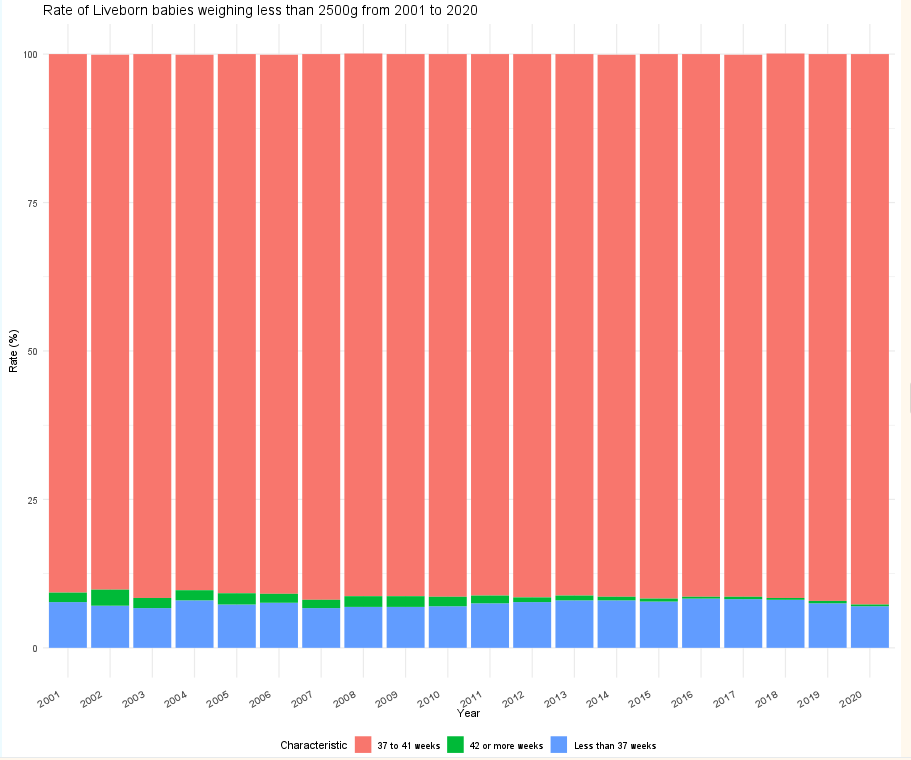
\includegraphics[width=0.8\textwidth]{subsections/baby_health/live_born_weigh_proportion_act.png}
  \caption{Liveborn baby weight proportion in ACT.}
  \label{fig:weight_gest}
\end{figure}

In \textbf{Figure \ref{fig:weight_act}} we can also see that even though the rate of underweight babies is around 5\% through the years it is showing an upward trend.

\begin{figure}
  \centering
  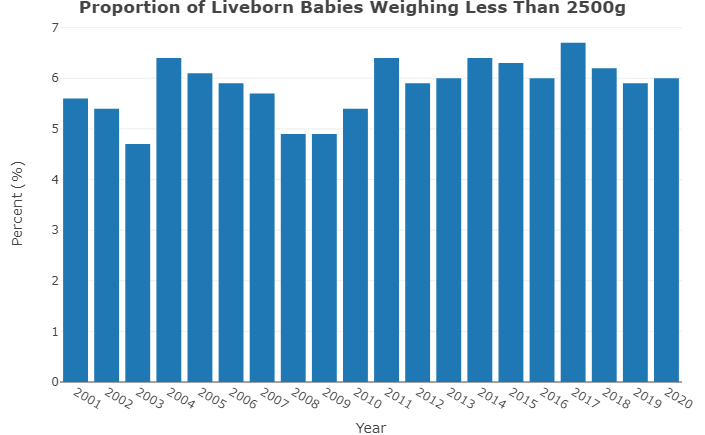
\includegraphics[width=0.8\textwidth]{subsections/baby_health/liveborn_weight.png}
  \caption{Underweight babies weight}
  \label{fig:weight_act}
\end{figure}